% 41039 Programming 1 revision; shared style copied from the established Week 4 deck.
\documentclass[aspectratio=169]{beamer}
\makeatletter

\usepackage{lmodern}
\usepackage{booktabs}
\usepackage{array}
\usepackage{graphicx}
\usepackage{xcolor}
\usepackage{listings}
\usepackage{pifont}
\usepackage{enumitem}
\usepackage[most]{tcolorbox}
\usepackage{tikz}
\usetikzlibrary{shapes.geometric, arrows.meta, positioning}

% Beamer's default enumerate label expands to itself once enumitem takes the optional
% argument, and TeX runs out of input stack. An explicit label breaks the loop.
\setlist[enumerate]{label=\arabic*.}
\setlist[itemize]{label=\usebeamertemplate{itemize item}}

\definecolor{bkblue}{RGB}{0,70,140}
\definecolor{bktitlebg}{RGB}{64,116,169}
\definecolor{codebg}{RGB}{244,246,249}
\definecolor{codecmt}{RGB}{110,120,130}
\definecolor{codegray}{RGB}{110,120,135}
\definecolor{codestr}{RGB}{150,60,20}
\definecolor{badred}{RGB}{185,40,40}
\definecolor{goodgreen}{RGB}{20,125,70}
\definecolor{srcgrey}{RGB}{105,115,128}

\usetheme{default}
\useinnertheme{rounded}
\setbeamertemplate{navigation symbols}{}

\setbeamercolor{titlelike}{bg=bktitlebg,fg=white}
\setbeamercolor{frametitle}{fg=bkblue,bg=}
\setbeamercolor{author}{fg=bkblue}
\setbeamercolor{institute}{fg=bkblue}
\setbeamercolor{section in toc}{fg=bkblue}
\setbeamerfont{frametitle}{size=\Large,series=\mdseries}
\setbeamerfont{title}{size=\Large,series=\bfseries}
\setbeamerfont{subtitle}{size=\normalsize,series=\bfseries}

\setbeamertemplate{frametitle}{%
  \vspace*{0.35em}%
  \begin{minipage}[b]{0.84\textwidth}%
    \usebeamerfont{frametitle}\usebeamercolor[fg]{frametitle}\insertframetitle%
  \end{minipage}\hfill%
  \begin{minipage}[b]{0.10\textwidth}%
    \raggedleft
\includegraphics[height=0.75cm]{bk-logo.png}%
  \end{minipage}\\[0.1em]%
  {\color{bkblue}\rule{\textwidth}{0.7pt}}%
}

\setbeamercolor{footbar}{bg=bkblue,fg=white}
\setbeamertemplate{footline}{%
  \begin{beamercolorbox}[wd=\paperwidth,ht=2.1ex,dp=1.1ex,leftskip=.3cm,rightskip=.3cm]{footbar}%
    \tiny\insertshorttitle\hfill\insertframenumber{}/\inserttotalframenumber%
  \end{beamercolorbox}%
}

\newcommand{\keyline}[1]{\vfill\begin{center}\textcolor{bkblue}{\textbf{#1}}\end{center}\vspace*{0.2em}}
\newcommand{\hd}[1]{\textbf{#1}}
\newcommand{\code}[1]{\texttt{#1}}
\newcommand{\srcline}[1]{{\color{srcgrey}\scriptsize #1\par}}
\newcommand{\srclink}[2]{\href{#1}{\texttt{#2}}}
\newcommand{\badlabel}[1]{\textcolor{badred}{\ding{55}~\textbf{#1}}}
\newcommand{\goodlabel}[1]{\textcolor{goodgreen}{\ding{51}~\textbf{#1}}}
\newcommand{\neutrallabel}[1]{\textcolor{bkblue}{\textbf{#1}}}
\newcommand{\timing}[2]{\hfill{\small\textcolor{bkblue}{\textbf{#1 \textbullet{} #2}}}}
% a blank to be filled in, numbered so the word bank can be checked against it
\newcommand{\blank}[1]{\underline{\hspace{1.1em}\textbf{(#1)}\hspace{1.1em}}}
\newcommand{\yes}{\textcolor{goodgreen}{\ding{51}}}
\newcommand{\no}{\textcolor{badred}{\ding{55}}}

% --- Stack and heap pictures (Draw it) --------------------------------------
\tikzset{
  sframe/.style={draw=bkblue, thick, fill=codebg, rounded corners=2pt, inner sep=4pt,
    font=\scriptsize\ttfamily, align=left, anchor=north west},
  ftitle/.style={font=\scriptsize\sffamily\bfseries, text=bkblue, anchor=south west},
  cell/.style={draw=bkblue, fill=white, font=\scriptsize\ttfamily, minimum width=0.62cm,
    minimum height=0.5cm, inner sep=1pt},
  atitle/.style={font=\scriptsize\ttfamily, text=bkblue, anchor=south west, inner sep=1pt},
  ref/.style={-{Stealth[length=5pt]}, thick, draw=bkblue!85!black},
  hd/.style={font=\small\sffamily\bfseries, text=bkblue},
}

\hypersetup{colorlinks=true, urlcolor=bkblue, linkcolor=bkblue}

% --- Question box: what the room is being asked --------------------------
\newtcolorbox{discussionbox}[1]{
  title=\textbf{#1}, coltitle=bkblue, colback=white, colframe=bkblue,
  colbacktitle=bkblue!10, boxrule=1pt, arc=3pt,
  left=6pt, right=6pt, top=4pt, bottom=4pt
}
% --- Answer box: revealed after they have committed to an answer ---------
\newtcolorbox{contextbox}[1]{
  title=\textbf{#1}, coltitle=white, colback=bkblue!5, colframe=bkblue,
  colbacktitle=bkblue!80, boxrule=0.6pt, arc=3pt,
  left=6pt, right=6pt, top=4pt, bottom=4pt
}

\lstdefinestyle{code}{
  basicstyle=\ttfamily\scriptsize,
  keywordstyle=\color{bkblue}\bfseries,
  commentstyle=\color{codecmt}\itshape,
  stringstyle=\color{codestr},
  backgroundcolor=\color{codebg},
  frame=leftline, framerule=1.2pt, rulecolor=\color{bkblue},
  xleftmargin=1.1em, framexleftmargin=1.1em,
  framexrightmargin=0.4em, framextopmargin=3pt, framexbottommargin=3pt,
  showstringspaces=false, columns=fullflexible, keepspaces=true,
  breaklines=true, aboveskip=0.6em, belowskip=0.6em,
}
\lstdefinestyle{bad}{style=code, rulecolor=\color{badred}, backgroundcolor=\color{badred!4}}
\lstdefinestyle{good}{style=code, rulecolor=\color{goodgreen}, backgroundcolor=\color{goodgreen!5}}
\lstset{style=code}
% listings' Python predates 3.10; teach it the soft keywords and constants this deck uses
\lstdefinelanguage{Py}[]{Python}{morekeywords={match,case,elif,True,False}}

\setbeamertemplate{title page}{%
  \vspace*{0.5em}
  \begin{centering}
    \begin{beamercolorbox}[sep=8pt,center,rounded=true,shadow=false]{title}
      \usebeamerfont{title}\inserttitle\par
      \ifx\insertsubtitle\@empty\else
        \vskip0.4em{\usebeamerfont{subtitle}\insertsubtitle\par}
      \fi
    \end{beamercolorbox}
    \vskip1.0em
    
\includegraphics[height=1.7cm]{bk-logo.png}
    \vskip1.0em
    {\usebeamercolor[fg]{author}\usebeamerfont{author}\insertauthor\par}
    \vskip0.5em
    {\usebeamercolor[fg]{institute}\usebeamerfont{institute}\insertinstitute\par}
    \vskip0.6em
    {\usebeamerfont{date}\insertdate\par}
  \end{centering}
}




\title[41039 Programming 1 --- Revision of Week 6]{41039 Programming 1}
\subtitle{Revision of Week 6: Building reliable classes}
\author{Dr. Xuan-Bach Le\\ \small\texttt{le.xuan.bach@hcmut.edu.vn}}
\institute{\small Faculty of Computer Science and Engineering, HCMUT}
\date{September Session 2026}
\AtBeginSection[]{\begin{frame}{Outline}\tableofcontents[currentsection]\end{frame}}
\begin{document}

\begin{frame}{}
\titlepage
\end{frame}

\begin{frame}{How the revision session works}
\begin{discussionbox}{A recap before the next lecture}\small Write an answer before the reveal. Explain the state change, rule or contract that makes it follow. These are practice questions, with no new assessment requirements.\end{discussionbox}
\begin{columns}[T,onlytextwidth]
\column{0.48\textwidth}
\raggedright
\neutrallabel{Part 1: on your own}\begin{itemize}\small\item 6 short questions\item About 90 seconds per question\item Java and Python; name the language first\end{itemize}
\column{0.48\textwidth}
\raggedright
\neutrallabel{Part 2: teams of 3 or 4}\begin{itemize}\small\item Draw the model\item Spot the errors\item Predict the output\item Write and test the code\end{itemize}
\end{columns}
\keyline{A result needs a reason. A repair needs a counterexample.}
\end{frame}

\section{On your own}

\begin{frame}[fragile]{1. A stock invariant}
\srcline{Java 8 excerpt: main statements and supporting types; commit to an outcome before the reveal.}
\begin{columns}[T,onlytextwidth]
\column{0.62\textwidth}
\raggedright
\begin{lstlisting}[style=code,language=Java]
Stock item = new Stock(4);
System.out.println(item.take(3));
System.out.println(item.take(2));
System.out.println(item.getStock());
class Stock {
    private int stock;
    Stock(int stock) { this.stock = stock; }
    boolean take(int amount) {
        if (amount <= 0 || amount > stock) return false;
        stock = stock - amount;
        return true;
    }
    int getStock() { return stock; }
}
\end{lstlisting}

\column{0.34\textwidth}
\raggedright
\begin{onlyenv}<1>\begin{discussionbox}{Your answer}\small What is the complete output? Which line or rule decides it?\end{discussionbox}\end{onlyenv}
\begin{onlyenv}<2>\begin{contextbox}{Answer}
\begin{lstlisting}[style=code]
true
false
1
\end{lstlisting}
\scriptsize\raggedright The first request leaves 1. The second request fails before changing the field, so it stays 1.
\end{contextbox}\end{onlyenv}
\end{columns}

\end{frame}

\begin{frame}[fragile]{2. The same contract in Python}
\srcline{Python 3; commit to an outcome before the reveal.}
\begin{columns}[T,onlytextwidth]
\column{0.62\textwidth}
\raggedright
\begin{lstlisting}[style=code,language=Py]
class Stock:
    def __init__(self, stock):
        self._stock = stock
    def take(self, amount):
        if amount <= 0 or amount > self._stock:
            return False
        self._stock -= amount
        return True
    def available(self):
        return self._stock
item = Stock(4)
print(item.take(3))
print(item.take(2))
print(item.available())
\end{lstlisting}

\column{0.34\textwidth}
\raggedright
\begin{onlyenv}<1>\begin{discussionbox}{Your answer}\small What is the complete output? Which line or rule decides it?\end{discussionbox}\end{onlyenv}
\begin{onlyenv}<2>\begin{contextbox}{Answer}
\begin{lstlisting}[style=code]
True
False
1
\end{lstlisting}
\scriptsize\raggedright Both languages implement the same rule. Python prints booleans with initial capitals.
\end{contextbox}\end{onlyenv}
\end{columns}

\end{frame}

\begin{frame}[fragile]{3. One object, two references}
\srcline{Java 8 excerpt: main statements and supporting types; commit to an outcome before the reveal.}
\begin{columns}[T,onlytextwidth]
\column{0.62\textwidth}
\raggedright
\begin{lstlisting}[style=code,language=Java]
Stock a = new Stock(5);
Stock b = a;
b.take(2);
System.out.println(a.getStock());
System.out.println(a == b);
class Stock {
    private int stock;
    Stock(int stock) { this.stock = stock; }
    void take(int amount) { stock -= amount; }
    int getStock() { return stock; }
}
\end{lstlisting}

\column{0.34\textwidth}
\raggedright
\begin{onlyenv}<1>\begin{discussionbox}{Your answer}\small What is the complete output? Which line or rule decides it?\end{discussionbox}\end{onlyenv}
\begin{onlyenv}<2>\begin{contextbox}{Answer}
\begin{lstlisting}[style=code]
3
true
\end{lstlisting}
\scriptsize\raggedright Assignment makes two names for one stock object. The mutation through b is visible through a.
\end{contextbox}\end{onlyenv}
\end{columns}

\end{frame}

\begin{frame}[fragile]{4. Separate objects, separate state}
\srcline{Python 3; commit to an outcome before the reveal.}
\begin{columns}[T,onlytextwidth]
\column{0.62\textwidth}
\raggedright
\begin{lstlisting}[style=code,language=Py]
class Basket:
    def __init__(self):
        self.items = []
a = Basket()
b = Basket()
a.items.append("tea")
print(a.items)
print(b.items)
print(a is b)
\end{lstlisting}

\column{0.34\textwidth}
\raggedright
\begin{onlyenv}<1>\begin{discussionbox}{Your answer}\small What is the complete output? Which line or rule decides it?\end{discussionbox}\end{onlyenv}
\begin{onlyenv}<2>\begin{contextbox}{Answer}
\begin{lstlisting}[style=code]
['tea']
[]
False
\end{lstlisting}
\scriptsize\raggedright Each constructor call allocates a separate items list; only a receives tea.
\end{contextbox}\end{onlyenv}
\end{columns}

\end{frame}

\begin{frame}[fragile]{5. Class count and instance number}
\srcline{Java 8 excerpt: main statements and supporting types; commit to an outcome before the reveal.}
\begin{columns}[T,onlytextwidth]
\column{0.62\textwidth}
\raggedright
\begin{lstlisting}[style=code,language=Java]
Ticket a = new Ticket();
Ticket b = new Ticket();
System.out.println(a.number + " " + b.number + " " + Ticket.count);
class Ticket {
    static int count = 0;
    final int number;
    Ticket() { number = ++count; }
}
\end{lstlisting}

\column{0.34\textwidth}
\raggedright
\begin{onlyenv}<1>\begin{discussionbox}{Your answer}\small What is the complete output? Which line or rule decides it?\end{discussionbox}\end{onlyenv}
\begin{onlyenv}<2>\begin{contextbox}{Answer}
\begin{lstlisting}[style=code]
1 2 2
\end{lstlisting}
\scriptsize\raggedright The shared counter reaches 2; a keeps its previously assigned number 1.
\end{contextbox}\end{onlyenv}
\end{columns}

\end{frame}

\begin{frame}[fragile]{6. A class attribute can share too much}
\srcline{Python 3; commit to an outcome before the reveal.}
\begin{columns}[T,onlytextwidth]
\column{0.62\textwidth}
\raggedright
\begin{lstlisting}[style=code,language=Py]
class Basket:
    items = []
a = Basket()
b = Basket()
a.items.append("tea")
print(b.items)
print(a.items is b.items)
\end{lstlisting}

\column{0.34\textwidth}
\raggedright
\begin{onlyenv}<1>\begin{discussionbox}{Your answer}\small What is the complete output? Which line or rule decides it?\end{discussionbox}\end{onlyenv}
\begin{onlyenv}<2>\begin{contextbox}{Answer}
\begin{lstlisting}[style=code]
['tea']
True
\end{lstlisting}
\scriptsize\raggedright Both objects find the class attribute. Move the list into \_\_init\_\_ to give each basket its own storage.
\end{contextbox}\end{onlyenv}
\end{columns}

\end{frame}

\section{Team round 1: draw the model}

\begin{frame}{Form teams}
\begin{itemize}[itemsep=0.8em]\item Teams of 3 or 4. One shared sheet, one spokesperson.\item For each challenge, record the result and the reason.\item Rotate the spokesperson. Other teams can challenge an explanation.\item The final task has starter files and a Java/Python solution pair.\end{itemize}\keyline{Discuss first. Commit to an answer. Then compare with the reveal.}
\end{frame}

\begin{frame}[fragile]{Draw it: References inside a composed object}
\begin{columns}[T,onlytextwidth]
\column{0.62\textwidth}
\raggedright
\begin{lstlisting}[style=code,language=Java]
Book book=new Book("Tea");
Shelf a=new Shelf(book);
Shelf b=a;
Shelf c=new Shelf(new Book("Coffee"));
b.book.title="Water";
System.out.println(a.book.title+" "+c.book.title);
System.out.println(a==b);
class Book { String title; Book(String t) { title=t; } }
class Shelf { Book book; Shelf(Book b) { book=b; } }
\end{lstlisting}

\column{0.34\textwidth}
\raggedright
\begin{discussionbox}{Four minutes}\small Draw the object references after the shown operations. Label the important state. Mark what is shared, what changes, or which path handles failure. Predict every output line.\end{discussionbox}
\end{columns}
\par\srcline{\href{../../weeks/week-6.html}{Course website: Week 6}. Complete programs accompany this deck.}

\end{frame}

\begin{frame}[fragile]{Draw it: one answer}
\begin{columns}[T,onlytextwidth]
\column{0.66\textwidth}
\raggedright
\resizebox{\linewidth}{!}{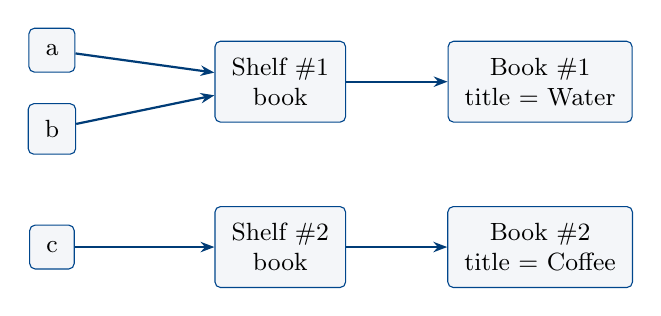
\begin{tikzpicture}
\node[draw=bkblue,rounded corners=2pt,fill=codebg,align=center,inner sep=6pt,font=\small] (a) at (0,0) {a};
\node[draw=bkblue,rounded corners=2pt,fill=codebg,align=center,inner sep=6pt,font=\small] (b) at (0,-1) {b};
\node[draw=bkblue,rounded corners=2pt,fill=codebg,align=center,inner sep=6pt,font=\small] (c) at (0,-2.5) {c};
\node[draw=bkblue,rounded corners=2pt,fill=codebg,align=center,inner sep=6pt,font=\small] (s1) at (2.9,-0.4) {Shelf \#1\\[0pt] book};
\node[draw=bkblue,rounded corners=2pt,fill=codebg,align=center,inner sep=6pt,font=\small] (s2) at (2.9,-2.5) {Shelf \#2\\[0pt] book};
\node[draw=bkblue,rounded corners=2pt,fill=codebg,align=center,inner sep=6pt,font=\small] (o1) at (6.2,-0.4) {Book \#1\\[0pt] title = Water};
\node[draw=bkblue,rounded corners=2pt,fill=codebg,align=center,inner sep=6pt,font=\small] (o2) at (6.2,-2.5) {Book \#2\\[0pt] title = Coffee};
\draw[ref] (a) -- (s1);
\draw[ref] (b) -- (s1);
\draw[ref] (c) -- (s2);
\draw[ref] (s1) -- (o1);
\draw[ref] (s2) -- (o2);
\end{tikzpicture}}

\column{0.3\textwidth}
\raggedright
\begin{contextbox}{Output}\begin{lstlisting}[style=code]
Water Coffee
true
\end{lstlisting}
\end{contextbox}
\end{columns}
\vspace{0.8em}
\small Two shelf objects and two book objects remain. a and b share the first shelf, which holds the renamed book.
\par\srcline{\href{../../weeks/week-6.html}{Course website: Week 6}. Complete programs accompany this deck.}

\end{frame}

\section{Team round 2: spot the errors}

\begin{frame}[fragile]{Spot the errors 1: Java (5 min)}
\begin{discussionbox}{Contract}\small take accepts a positive amount no larger than stock, preserves state on rejection, and reports success truthfully.\end{discussionbox}
\begin{columns}[T,onlytextwidth]
\column{0.48\textwidth}
\raggedright
\begin{lstlisting}[style=bad,language=Java,numbers=left,numberstyle=\tiny\color{codegray},firstnumber=1,numbersep=0.7em]
public class Broken {
    public static void main(String[] args) {
        Stock s=new Stock(4);
        System.out.println(s.take(0));
        System.out.println(s.take(4));
        System.out.println(s.take(1));
        System.out.println(s.left());
    }
}
class Stock {
\end{lstlisting}

\column{0.48\textwidth}
\raggedright
\begin{lstlisting}[style=bad,language=Java,numbers=left,numberstyle=\tiny\color{codegray},firstnumber=11,numbersep=0.7em]
    private int count;
    Stock(int count) { this.count=count; }
    boolean take(int n) {
        if(n<0 || n>=count) return false;
        count-=n;
        return false;
    }
    int left() { return count; }
}
\end{lstlisting}

\end{columns}

\end{frame}

\begin{frame}[fragile]{Spot the errors 1: answers}
\begin{columns}[T,onlytextwidth]
\column{0.58\textwidth}
\raggedright
\begin{contextbox}{The repairs}\footnotesize\begin{itemize}[itemsep=0.45em]\item \textbf{L14:} Reject n \textless{}= 0, but allow n exactly equal to the available stock.\item \textbf{L16:} The successful mutation must return true. The rejection branch still returns false.\end{itemize}\end{contextbox}
\column{0.38\textwidth}
\raggedright
\badlabel{Original program}\begin{lstlisting}[style=code]
false
false
false
3
\end{lstlisting}
\goodlabel{After the repairs}\begin{lstlisting}[style=code]
false
true
false
0
\end{lstlisting}

\end{columns}
\par\srcline{\href{../../weeks/week-6.html}{Course website: Week 6}. Complete programs accompany this deck.}

\end{frame}

\begin{frame}[fragile]{Spot the errors 2: Python (5 min)}
\begin{discussionbox}{Contract}\small copy must make an independent basket. Adding milk to b must leave a with tea only.\end{discussionbox}
\begin{columns}[T,onlytextwidth]
\column{0.48\textwidth}
\raggedright
\begin{lstlisting}[style=bad,language=Py,numbers=left,numberstyle=\tiny\color{codegray},firstnumber=1,numbersep=0.7em]
class Basket:
    def __init__(self): self.items=[]
    def copy(self): return self
    def add(self,name): self.items.append(name)
    def count(self): print(len(self.items))
\end{lstlisting}

\column{0.48\textwidth}
\raggedright
\begin{lstlisting}[style=bad,language=Py,numbers=left,numberstyle=\tiny\color{codegray},firstnumber=7,numbersep=0.7em]
a=Basket()
a.add("tea")
b=a.copy()
b.add("milk")
print(a.items,b.items)
print(a.count())
\end{lstlisting}

\end{columns}

\end{frame}

\begin{frame}[fragile]{Spot the errors 2: answers}
\begin{columns}[T,onlytextwidth]
\column{0.58\textwidth}
\raggedright
\begin{contextbox}{The repairs}\footnotesize\begin{itemize}[itemsep=0.45em]\item \textbf{L3:} Construct a distinct basket and copy the items list.\item \textbf{L5:} Return the count instead of printing and returning None.\end{itemize}\end{contextbox}
\column{0.38\textwidth}
\raggedright
\badlabel{Original program}\begin{lstlisting}[style=code]
['tea', 'milk'] ['tea', 'milk']
2
None
\end{lstlisting}
\goodlabel{After the repairs}\begin{lstlisting}[style=code]
['tea'] ['tea', 'milk']
1
\end{lstlisting}

\end{columns}
\par\srcline{\href{../../weeks/week-6.html}{Course website: Week 6}. Complete programs accompany this deck.}

\end{frame}

\section{Team round 3: predict the output}

\begin{frame}[fragile]{Predict 1: Shared count, separate counts}
\begin{columns}[T,onlytextwidth]
\column{0.62\textwidth}
\raggedright
\begin{lstlisting}[style=code,language=Java]
Counter a=new Counter();
Counter b=new Counter();
a.click(); b.click(); b.click();
Counter c=b;
c.click();
System.out.println(a.mine+" "+b.mine+" "+Counter.total);
System.out.println(c==b);
class Counter {
    static int total=0;
    int mine=0;
    void click() { total++; mine++; }
}
\end{lstlisting}

\column{0.34\textwidth}
\raggedright
\begin{discussionbox}{Three minutes}\small Write every line in order. Explain the first state change, alias, dispatch decision or exception that controls the result. Then propose one change that alters the output.\end{discussionbox}
\end{columns}
\par\srcline{\href{../../weeks/week-6.html}{Course website: Week 6}. Complete programs accompany this deck.}

\end{frame}

\begin{frame}[fragile]{Predict 1: answer}
\begin{columns}[T,onlytextwidth]
\column{0.42\textwidth}
\raggedright
\begin{lstlisting}[style=code]
1 3 4
true
\end{lstlisting}

\column{0.54\textwidth}
\raggedright
\begin{contextbox}{Why}\small There are two Counter objects and four clicks. c aliases b rather than constructing another counter.\end{contextbox}
\end{columns}
\par\srcline{\href{../../weeks/week-6.html}{Course website: Week 6}. Complete programs accompany this deck.}

\end{frame}

\begin{frame}[fragile]{Predict 2: Mutation followed by shadowing}
\begin{columns}[T,onlytextwidth]
\column{0.62\textwidth}
\raggedright
\begin{lstlisting}[style=code,language=Py]
class Basket:
    items=[]
a,b=Basket(),Basket()
a.items.append("tea")
b.items=["coffee"]
a.items.append("milk")
print(a.items)
print(b.items)
print(Basket.items)
\end{lstlisting}

\column{0.34\textwidth}
\raggedright
\begin{discussionbox}{Three minutes}\small Write every line in order. Explain the first state change, alias, dispatch decision or exception that controls the result. Then propose one change that alters the output.\end{discussionbox}
\end{columns}
\par\srcline{\href{../../weeks/week-6.html}{Course website: Week 6}. Complete programs accompany this deck.}

\end{frame}

\begin{frame}[fragile]{Predict 2: answer}
\begin{columns}[T,onlytextwidth]
\column{0.42\textwidth}
\raggedright
\begin{lstlisting}[style=code]
['tea', 'milk']
['coffee']
['tea', 'milk']
\end{lstlisting}

\column{0.54\textwidth}
\raggedright
\begin{contextbox}{Why}\small Appending changes the shared class list. Assigning b.items creates a separate instance attribute for b.\end{contextbox}
\end{columns}
\par\srcline{\href{../../weeks/week-6.html}{Course website: Week 6}. Complete programs accompany this deck.}

\end{frame}

\section{Team round 4: write the code}

\begin{frame}[fragile]{Code it: specification}
\begin{discussionbox}{An inventory that preserves its invariant}\small Read the initial stock, n, then n requests, with each input value on a separate line. Accept positive requests no larger than the remaining stock. Print OK or Refused after each request, then the final stock. Rejecting a request must leave stock unchanged.\end{discussionbox}
\begin{columns}[T,onlytextwidth]
\column{0.48\textwidth}
\raggedright
\neutrallabel{Example input}\begin{lstlisting}[style=code]
5
4
2
4
0
3
\end{lstlisting}

\column{0.48\textwidth}
\raggedright
\neutrallabel{Expected output}\begin{lstlisting}[style=code]
OK
Refused
Refused
OK
0
\end{lstlisting}

\end{columns}
\small Eight minutes. One Java team and one Python team at the keyboard. Other teams produce a boundary test and explain which wrong implementation it would expose.
\end{frame}

\begin{frame}[fragile]{Code it: Java solution}
\begin{lstlisting}[style=code,language=Java,numbers=left,numberstyle=\tiny\color{codegray},firstnumber=1,numbersep=0.7em]
java.util.Scanner sc = new java.util.Scanner(System.in);
Inventory item = new Inventory(sc.nextInt());
int n = sc.nextInt();
for (int i=0;i<n;i++) System.out.println(item.take(sc.nextInt()) ? "OK" : "Refused");
System.out.println(item.available());
class Inventory {
    private int stock;
    Inventory(int stock) { this.stock = stock; }
    boolean take(int amount) {
        if (amount <= 0 || amount > stock) return false;
        stock -= amount;
        return true;
    }
    int available() { return stock; }
}
\end{lstlisting}
\par\srcline{\href{../../weeks/week-6.html}{Course website: Week 6}. Complete programs accompany this deck.}

\end{frame}

\begin{frame}[fragile]{Code it: Python solution}
\begin{lstlisting}[style=code,language=Py,numbers=left,numberstyle=\tiny\color{codegray},firstnumber=1,numbersep=0.7em]
class Inventory:
    def __init__(self, stock): self._stock = stock
    def take(self, amount):
        if amount <= 0 or amount > self._stock: return False
        self._stock -= amount
        return True
    def available(self): return self._stock
item = Inventory(int(input()))
n = int(input())
for _ in range(n):
    print("OK" if item.take(int(input())) else "Refused")
print(item.available())
\end{lstlisting}
\par\srcline{\href{../../weeks/week-6.html}{Course website: Week 6}. Complete programs accompany this deck.}

\end{frame}

\begin{frame}{Code it: the tests}
\footnotesize {\scriptsize A slash separates input lines; (blank) denotes an empty line.\par}\medskip \textbf{Test 1}\par \code{5 / 4 / 2 / 4 / 0 / 3}\par \textbf{Output:} \code{OK / Refused / Refused / OK / 0}\par\medskip \textbf{Test 2}\par \code{0 / 2 / 1 / -1}\par \textbf{Output:} \code{Refused / Refused / 0}\par\medskip \textbf{Test 3}\par \code{3 / 0}\par \textbf{Output:} \code{3}\par\medskip \keyline{Explain why each test is present, not only whether it passes.}
\end{frame}

\section{Wrapping up}

\begin{frame}{What you should now be able to explain}
\begin{itemize}[itemsep=0.6em]\item State an invariant and check every mutating path.\item Distinguish copying a reference from copying a model.\item Place per-object mutable data in each instance.\item Use composition and narrow methods to preserve rules.\end{itemize}\vfill\small Return to the matching week page for runnable examples and further practice. Bring one unresolved prediction or counterexample to the next class.\par\srcline{\href{../../weeks/week-6.html}{Course website: Week 6}. Complete programs accompany this deck.}

\end{frame}

\end{document}
